\chapter{Propagacja}

\section{Układ}

\begin{itemize}
    \item Schemat układu wraz z rozpiską pinów
        \begin{figure}[H]
            \centering
            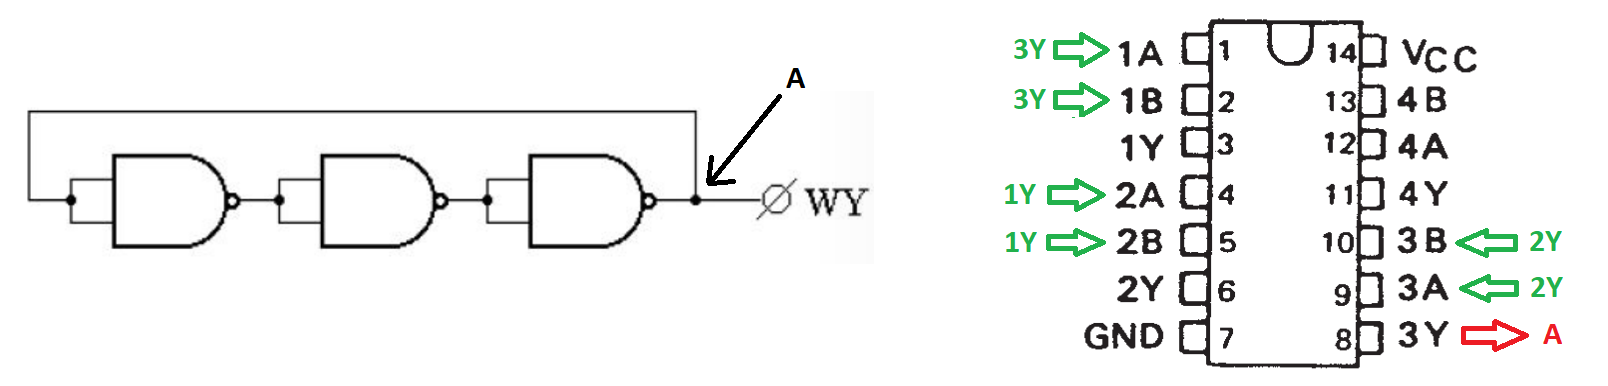
\includegraphics[width=\textwidth]{img/schemes_with_pins/propagacja_w_pins.png}
            \caption{Schemat układu}
            \label{propagacja:schemat}
        \end{figure}
        
    \item Złożony układ:
        \begin{figure}[H]
            \centering
            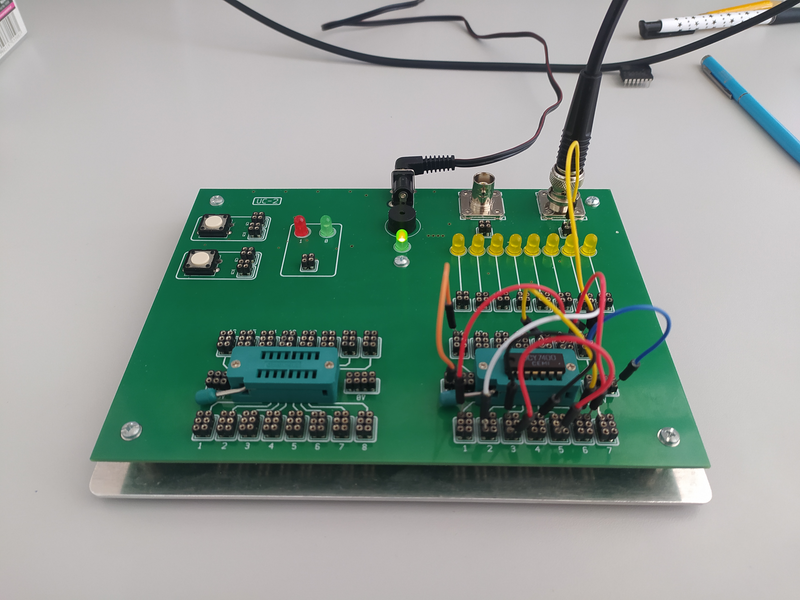
\includegraphics[width=\textwidth]{img/propagacja/1652306732374_scaled.png}
            \caption{Złożony układ}
            \label{propagacja:zlozony_uklad}
        \end{figure}
\end{itemize}

\pagebreak

\section{Pomiary}

\begin{itemize}
    \item Pomiary przeprowadzono dla układu \textbf{TTL 7400}, oraz \textbf{74S00}. Układy posiadają takie samo rozłożenie pinów, dzięki czemu należało wymienić tylko zamocowany układ aby przeprowadzić pomiar dla w/w układów.
    \item Dla układu \textbf{TTL 7400}:
        \begin{figure}[H]
            \centering
            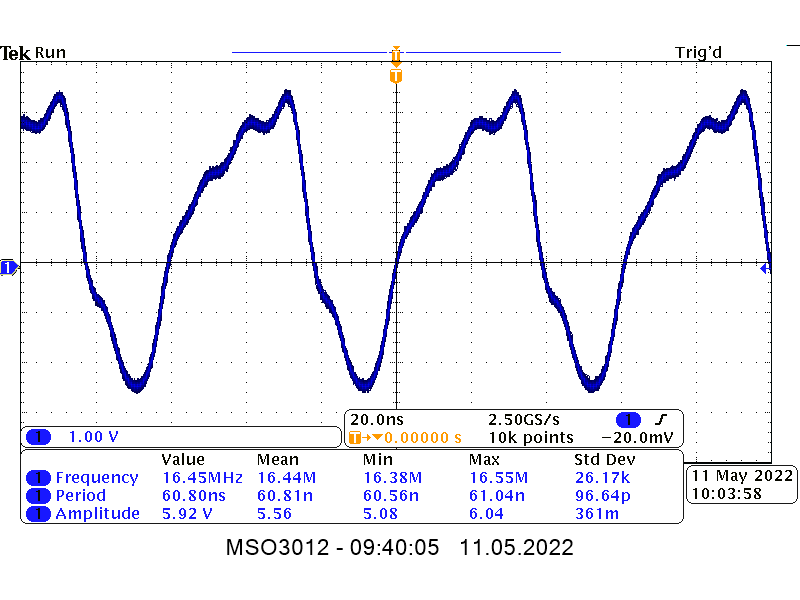
\includegraphics[width=0.7\textwidth]{img/osciloscope/4_propagacja.png}
            \caption{Ściągnięty okres dla układu TTL 7400}
            \label{propagacja:okres_7400}
        \end{figure}
        Teoretyczny średni czas propagacji wynosi (patrz: \ref{propagacja:sredni_czas}, \ref{dokumentacja:7400}):
            \begin{equation}
                t_{teor} = \dfrac{15ns + 22ns}{2} = \textbf{18.5ns}
            \end{equation}
        Okres wyniósł:
            \begin{center}
                $T_{7400}$ = \textbf{60.81ns}
            \end{center}
        Średni czas propagacji:
            \begin{equation}
                t_p = \dfrac{T_{7400}}{6} = \dfrac{60.81ns}{6} \approx \textbf{10.13ns}
            \end{equation}
           
\pagebreak
           
    \item Dla układu \textbf{TTL 74S00}:
        \begin{figure}[H]
            \centering
            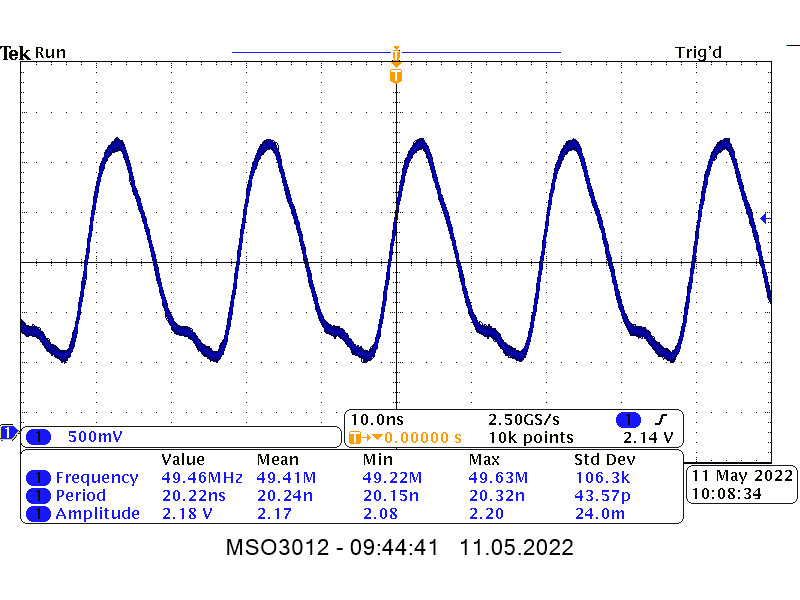
\includegraphics[width=0.7\textwidth]{img/osciloscope/4_propagacja74S00.png}
            \caption{Ściągnięty okres dla układu TTL 74S00}
            \label{propagacja:okres_74S00}
        \end{figure}
        Teoretyczny średni czas propagacji wynosi (patrz: \ref{propagacja:sredni_czas}, \ref{dokumentacja:74S00}):
            \begin{equation}
                t_{teor} = \dfrac{4.5ns + 5ns}{2} = \textbf{4.75ns}
            \end{equation}
        Okres wyniósł:
            \begin{center}
                $T_{74S00}$ = \textbf{20.24ns}
            \end{center}
        Średni czas propagacji:
            \begin{equation}
                t_p = \dfrac{T_{74S00}}{6} = \dfrac{20.24ns}{6} \approx \textbf{3.37ns}
            \end{equation}
\end{itemize}